\documentclass{article}
\usepackage{bigstrut}
\usepackage{adjustbox}
\usepackage{graphicx}^^M
\graphicspath{ {images/} }
\usepackage[T1]{fontenc}
\usepackage{float}

\usepackage[english]{babel}
\usepackage[utf8]{inputenc}
\usepackage{indentfirst}

\addtolength{\oddsidemargin}{-.875in}
\addtolength{\evensidemargin}{-.875in}
\addtolength{\textwidth}{1.75in}
\addtolength{\textheight}{1in}

\begin{document}
\title{Design V: Lab 7}
\begin{titlepage}
    \centering
	{\scshape\LARGE Lab 7: Sn-Bi Phase Diagram Analysis\par}
	\vspace{1cm}
	{\scshape Alex Smith: Recorder \hfill ID\#:10416940 \par}
	{\scshape Marcin Wisniowski: Manager \hfill ID\#:10417225\par}
	{\scshape Naomi Henderson: Technician \hfill ID\#:10406469\par}
    \vfill
	{\scshape Design V, Week 5\par}
	\vspace{.5cm}
	{\scshape Laboratory Performed: March 6th, 2018\\Stevens Institute of Technology\\E-231 Section I Group 1\par}
	\vspace{.5cm}
	{\scshape supervised by\\Mr. Di Wu, Mr. Kai Zong \par}
    \vfill
% Bottom of the page
	{\scshape“I pledge my honor that I have abided by the Stevens Honor System.”\par}
	\vspace{.5cm}
	{\scshape Alex Smith \hfill Date: 03/4/18\\Marcin Wisniowski \hfill Date: 03/4/18\\ Naomi Henderson \hfill Date: 03/4/18\\}
	\vspace{3cm}
\end{titlepage}

\section{Introduction}
In this lab, the group was tasked to learn about materials through their properties when cooled as well as their phase diagrams. A phase is defined as a homogeneous portion of matter with a distinct chemical composition and uniform physical properties which is also physically separable from its surroundings. A phase diagram is also useful in differentiating properties. A phase diagram allows the group to map the phase or phases which are present as a function of different thermodynamic variables. The design of engineering materials frequently makes use of phase diagrams in order to design and predict the micro-structures of a material subject to a specific set of processing conditions. In this case, the properties of Tin and Bismuth can be dramatically changed by adding a second phase into the micro-structure. Parts of the Sn-Bi phase diagram will be observed through the cooling of the samples that are given. 

\subsection{Objectives}
\begin{enumerate}
\item Use a phase diagram to design different micro-structures and relate those micro-structures to properties required for particular applications
\item Determine the phase or phases present, their compositions, and their relative amounts, given a specific coordinate pair on a phase diagram.
\item Sketch a typical cooling curve characterizing the change in temperature of an alloy specimen as a function of time as the specimen is cooled from above its melting temperature to room temperature
\item Use an optical microscope and briefly describe the basic properties of its operation
\end{enumerate}

\subsection{Hypothesis}
The group believes that as more Bismuth is found within the sample, the longer the cooling will take until stability. Similarly, the properties of the material will deviate from each other when cooled with different compositions. 

\section{Procedure}
\subsection{Cooling Data Collection}
The group initially needed to learn how to collect cooling data in order to later use this data for analysis. Using a computerized DAQ system (Capstone), cooling data could be found for various Sn-Bi mixtures. To set up the device, the "Table \& Graph" template was chosen and the x-axis and y-axis were set to Time and Temperature. Finally, the recording rate was set to 1 Hz (1 point per second).

\subsection{Melting Alloys}
After setting up the Capstone machine, the group received a specific Sn-Bi sample to record cooling data for. The sample was connected to the Capstone machine through a thermistor and the test tube containing the sample was lowered into a molten bath. After the metal appeared to no longer increase in temperature, the test tube was raised out of the molten bath and the cooling data was recorded until the sample seemed to longer change in temperature. 

\subsection{Optical Microscope}
Finally, while waiting for the cooling data to collect, the group used an optical microscope to observe the micro-structures at a magnification of 10x and 60x to see how they differed with different compositions. Each of the three samples was captured through the MotiConnection application and observations were made about their differences. 

\section{Results}
\subsection{Cooling Curve Plots}
\begin{center}
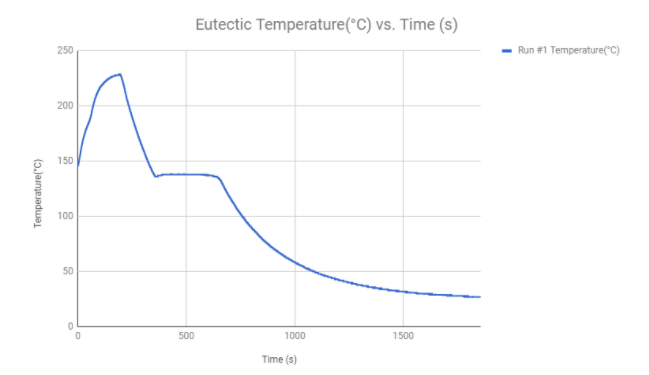
\includegraphics[width=400pt]{Eutectic_Graph.png}
\end{center}
The eutectic temperature vs time graph shows two sections of the material changing in slope. At the beginning, the change is steep, until it goes through a phase change where the temperature does not change, and again begins to drop off, slower.


\begin{center}
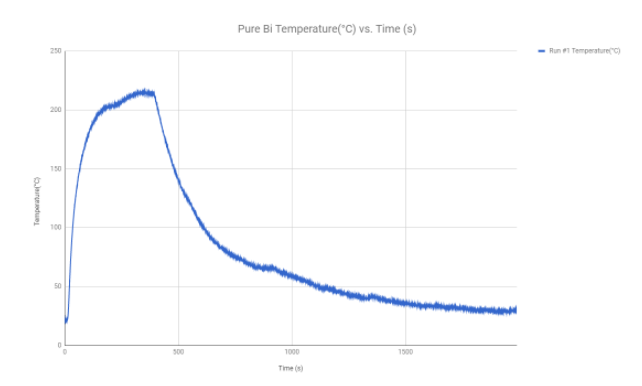
\includegraphics[width=400pt]{PureBi_Graph.png}
\end{center}
For the pure Bi, the cooling curve shows that the melting temperature of Bi is about 200$^o$C, where it turns from a solid to a liquid. The steep negative slope, where the Bi begins to cool (around 400 seconds), indicates the cooling rate. The slope begins to decrease as the the Bi sample tries to reach its equilibrium freezing temperature and turns from a liquid back to a solid. It can be seen in the graph that the Bi transitions from a liquid to a solid at about 950 seconds at roughly 70$^o$C. 



\begin{center}
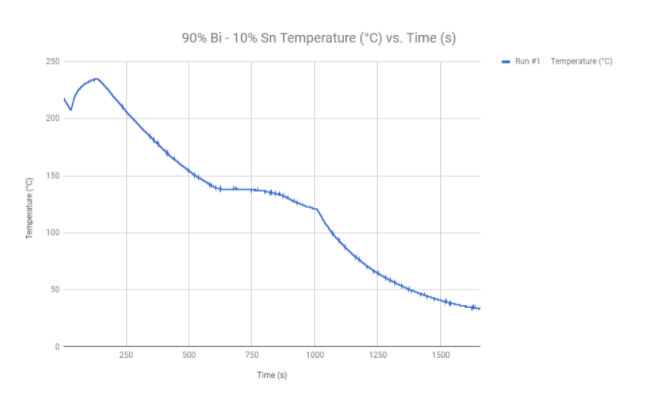
\includegraphics[width=400pt]{90Bi10Sn_Graph.png}
\end{center}
The 90\% Bi- 10\% Sn Temperature vs Time graph shows three distinct slopes through its cooling process. At the start the slope is steeper, until ~600 seconds, when there is a  slight stop in temperature change. The composition then drops in temperature at a slower rate, until around ~1000 seconds when it enters its 3rd phase.  


\begin{center}
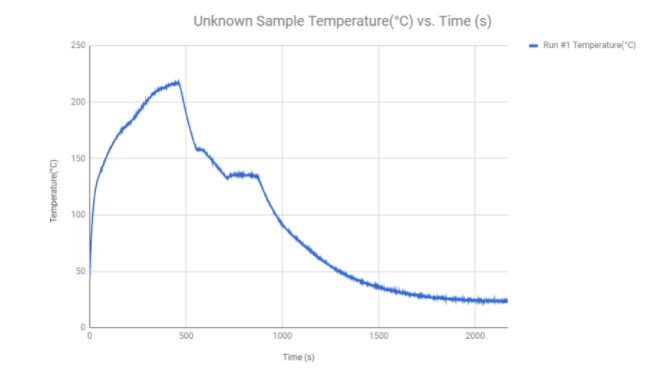
\includegraphics[width=400pt]{UnknownSample_Graph.png}
\end{center}
The unknown sample sees three distinct temperature vs time slopes, with a certain time frame with no temperature change. The slopes start steep at around ~500 seconds, but quickly enter the second phase within under a minute. The slope then gets less steep, levels off again, and changes one final time around ~800 seconds. 

\subsection{Phase Diagram Inflection Points}

\begin{center}
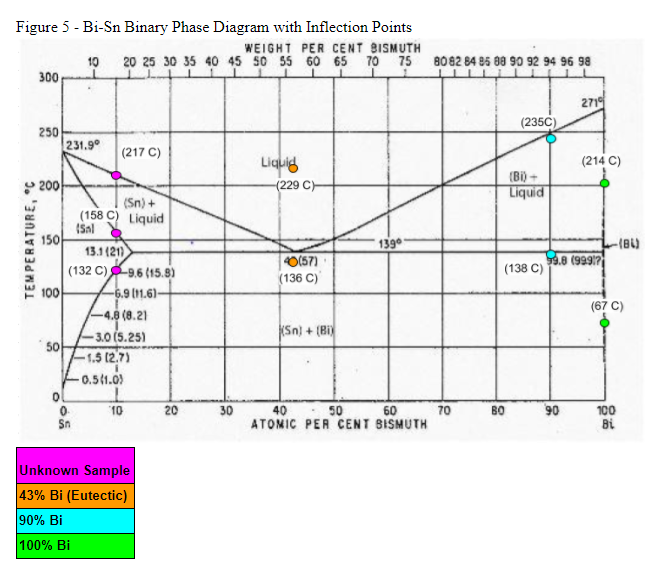
\includegraphics[width=400pt]{PhaseDiagram.png}
\end{center}

The inflection points were placed on the graph above based on when the slope of each cooling curve changed. The values fit strongly to the curve, except for 100\% Bismuth which may not have been allowed to heat up fully before the cooling process began. In the end, the unknown sample was shown to be 10\% Bismuth - 90\% Tin, and it fit with little error in the phase diagram above. 

\subsection{Metallography Observations}

\begin{center}
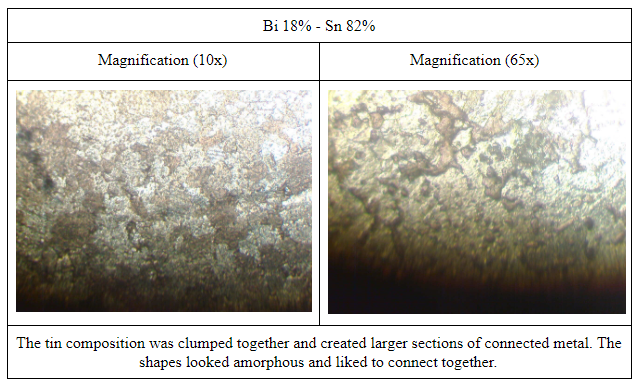
\includegraphics[width=400pt]{Microscope18Bi82Sn.png}
\end{center}

\begin{center}
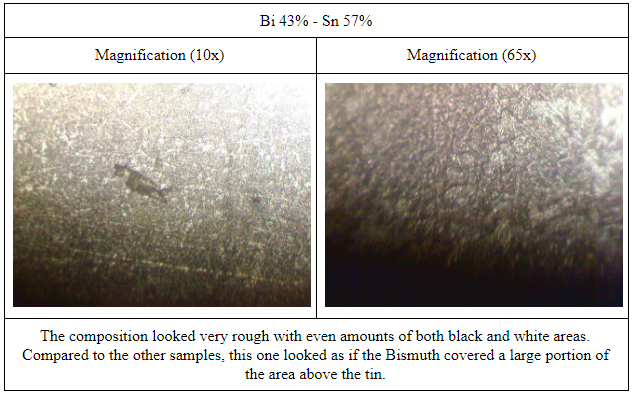
\includegraphics[width=400pt]{Microscope43Bi57Sn.png}
\end{center}

\begin{center}
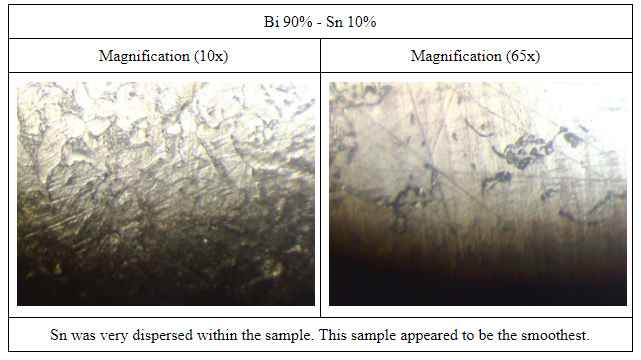
\includegraphics[width=400pt]{Microscope90Bi10Sn.png}
\end{center}

\section{Discussion}
The group learned the importance of phase diagrams and how different compositions of materials change the overarching properties of that material. By using a phase diagram, the group was easily able to differentiate the relationship between temperature and composition in the cooling of the samples. When looking closely at the structures through the microscope, the group was even able to differentiate the different types of phases, including the pro-eutectic and eutectic areas of each of the samples. 

Furthermore, the group was able to experimentally determine the melting temperatures of different samples and graphically see when the solidification process occurred in each. For instance, in 18\% Bi and 82\% Sn, while the liquid starts to become a solid at around 180 $^o$C, the eutectic solidification only begins to occurs at 138, showing a smoother surface than the 43\% and 57\% Sn sample. Finally, the group hypothesis was disproved through the experimentations conducted. Initially, the group believed that adding more bismuth would increase the melting point, because it had a higher melting temperature, but the melting point actually followed two separate linear correlations depending on the percent of composition. 


\section{Broader Impacts}
\begin{enumerate}
\item Using the micro-structures recorded in class (as a reference) estimate the composition of the alloy in the micro-structure at right. Is the alloy to the Bismuth rich or tin rich side of the eutectic composition?
\paragraph{}
The given micro-structure most resembles the Bi 18\% - Sn 82\% alloy, but seems to contain less tin. Therefore the micro-structure in the picture could have a composition of Bi 30\% - Sn 70\%. The sample is to the tin rich side of the eutectic composition, or left of the eutectic point.

\item Eutectic alloys have many useful applications. For example 60/40 Lead/Tin alloys were widely used as solders for both plumbing and electrical applications until environmental and health concerns precluded their used (although they are still widely available). Why might this eutectic alloy be so useful? Consider but their melting temperature and solidification behavior. Use the Internet to find several “lead-free” solder compositions. What is one such composition? Where is it used(what application)? How does it compare to lead tin?
\paragraph{}
The alloy composed of Sn 60\% - Pb 40\% was once very commonly used in soldering processes for both electrical and plumbing applications. The high tin content lowers the melting point of the alloy to a value easily attainable by standard soldering irons. Therefore, a greater tin composition also increases the workability and paste-like properties of the solder (Davis, Alloying). The tin fraction allows workers to spread the solder very easily in order to get the coverage and effectiveness they need in their work. The lead is the cheaper, higher melting point metal in the alloy. A greater lead concentration yields a more solid solder that does not spread as far and stays where the worker wants it (Davis, Alloying). More lead also means there will be more solid particles in the pasty solder, and the heat capacity of lead means that it takes more time to fully solidify, which allows the solder to more properly settle into its desired location.

Due to health and environmental concerns, lead usage in common solder is no longer viable. A popular new alternative is a blend of silver, copper, and tin, specifically 95.5\% Sn - 3.9\% Ag - 0.6\% Cu (Lead-Free Solder FAQ’s). The blend, one of the so called SAC family, is utilized in electrical work and circuit linkage. This alloy has a higher melting point than 60/40 Sn/Pb, melting between 217 - 225 degrees Celsius (FAQ’s). However, it also has a large modulus of elasticity, large yield strength, and decent workability, making it an attractive alternative to lead (Sawamura and Takeo, “Difference Between Various Sn/Ag/Cu Solder Compositions”).

\end{enumerate}

\section{References}
\begin{enumerate}
\item Capstone computer software for temperature graphs
\item MotiConnection application for optical microscope
\item Joseph R. Davis (2001). Alloying: Understanding the Basics. ASM International. p. 538.
Lead-Free Solder FAQ’s. Archived October 15, 2006, at the Wayback Machine.
\item Sawamura, Tadashi; Igarashi, Takeo (2005-06-29). "Difference Between Various Sn/Ag/Cu 
Solder Compositions" (PDF). Almit Ltd. Retrieved 2016-08-24.

\end{enumerate}
\end{document}